%%%% CAPÍTULO 3 - MATERIAL E MÉTODOS (PODE SER OUTRO TÍTULO DE ACORDO COM O TRABALHO REALIZADO)

\chapter{Materiais e Metodologia}\label{cap:materialemetodos}

Neste capítulo, serão discutidos e analisados todos os processos relacionados com o desenvolvimento do protótipo, a justificativa de cada escolha tomada, assim como um \textit{\gls{BOM}} (\textit{Bill of Materials}) consolidado, com os preços na data do trabalho, para a confecção de um protótipo.

\section{Metodologia}\label{sec:metodo}

Esta seção será dedicada à discussão sobre todas as partes integrantes do protótipo.

\subsection{Circuito}\label{circuit}

O circuito foi projetado para seguir um fluxo de informações conforme o diagrama de blocos representado na \autoref{fig:dflux}. Baseando-se na pesquisa apresentada no \autoref{cap:referencialTeorico}, este fluxo foi feito para guiar a lógica de design e também para explicar sucintamente o que cada parte do sistema compreende.

\begin{figure}[htb!]
    \caption{Diagrama de Blocos da Lógica de Funcionamento}
    \label{fig:dflux}
    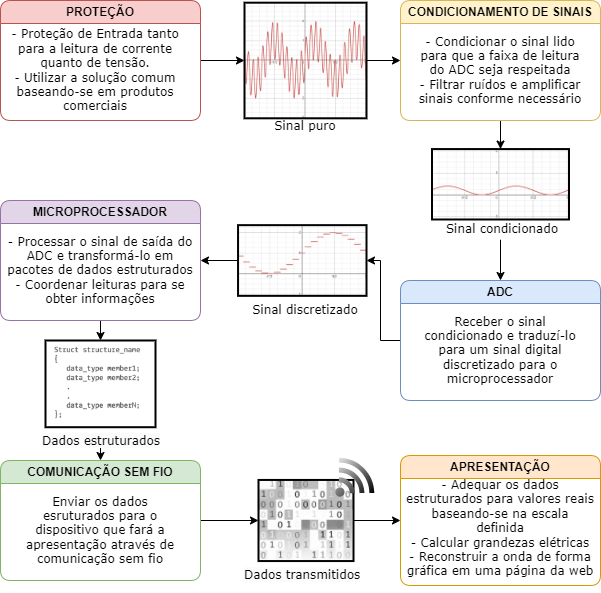
\includegraphics[width=1.0\textwidth]{figuras/dblocflux.png}
    \fonte{}
\end{figure}

Primeiramente, se tem a proteção de entrada. Esta é dividida em duas partes, sendo uma delas a proteção da entrada da tensão e a outra da corrente. Para se proteger a entrada de tensão, utilizam-se um resistor \gls{PTC} e \gls{MOV}s. O \gls{PTC} é projetado para caso a tensão de entrada do circuito seja muito maior que a desejada ou tenha um curto, este esquente e vire uma impedância muito grande, sendo assim uma barreira para qualquer tipo de corrente. Porém, a sua atuação para proteção é demasiada lenta, se pondo necessário a implementação dos \gls{MOV}s, que atuarão mais rapidamente e fecharão um curto entre a entrada e o ground do circuito enquanto o resistor está sendo ativado.

Para a proteção de corrente, utiliza-se primeiramente fusíveis \gls{HRC}, que são fusíveis especiais projetados para extinguir qualquer possível arco voltaico resultante da queima do filamento interno. Isso evita a continuidade da corrente após a atuação do fusível.

Em seguida, a ponte de diodos, posicionada logo após os resistores shunt, atua como um limitador de tensão (clamp) para evitar que a tensão ultrapasse os valores desejados. Além disso, ela proporciona um caminho para a corrente quando esta não é suficiente para queimar os fusíveis, mas pode danificar o circuito.

A disposição desses componentes e sua montagem estão detalhadas na \autoref{fig:circ-prot}.

\begin{figure}[htb!]
    \caption{Entrada de Tensão e Corrente}
    \label{fig:circ-prot}
    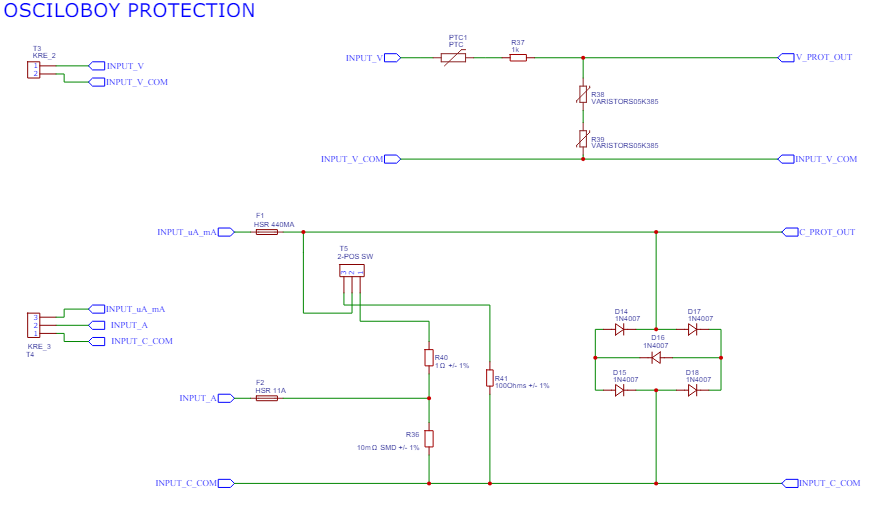
\includegraphics[width=1.0\textwidth]{figuras/circ-prot.png}
    \fonte{}
\end{figure}

Nesta figura, também é possível observar as entradas do circuito. A entrada de tensão está diretamente conectada à próxima etapa, responsável pelo condicionamento dos sinais de tensão. Já a entrada de corrente é composta por resistores que atuam como shunts (R41, R36 e R41), permitindo a leitura da corrente.

O resistor de 10 m$\Omega$ é para a leitura de corrente na proporção de Amperes, a série entre este e o resistor de 1 $\Omega$ compõe a leitura da entrada de mA e o resistor de 100 $\Omega$ para a leitura de $\mu$A. Para alternar entre as entradas de mA/$\mu$A e A, foi colocada uma chave mecânica de duas posições.

Para se obter um sinal apropriado para o ADC, existem duas possibilidades: leitura "Diferencial" e leitura "\textit{Single-Ended}".

\subsubsection{ADC - Modo \textit{Single-Ended}}\label{single-ended}

A primeira opção a ser considerada foi a \textit{Single-Ended}. Este tipo de leitura é feita pela comparação de tensão entre um ponto do circuito e o \textit{ground}. Para fazer tal leitura com diferentes \textit{ranges}, o que é fundamental para se alcançar uma boa precisão, foi primeiro projetado um condicionamento de sinais por divisor resistivo, como representado na \autoref{fig:div-res}.

\begin{figure}[htb!]
    \caption{Condicionamento de sinais por divisor resistivo para leitura \textit{Single-Ended}}
    \label{fig:div-res}
    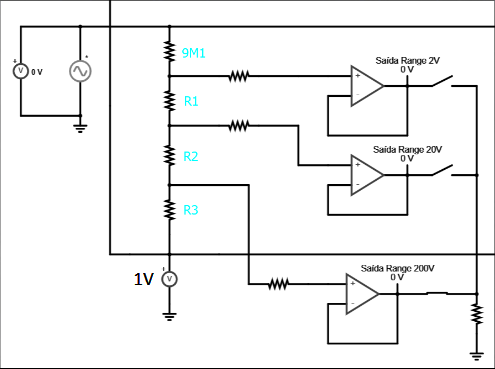
\includegraphics[width=0.6\textwidth]{figuras/div-res.png}
    \fonte{}
\end{figure}

Esta topologia promete 4 ranges de leitura tanto para corrente quanto para tensão, sendo estes 200 V, 20 V, 2 V e 200 mV e 10 A, 200 mA, 20 mA e 2000 $\mu$A. É também necessário o uso de \gls{amp-op}s para a seleção do range, para isolar o \gls{ADC} da entrada e também para manter a tensão de entrada do \gls{ADC} dentro do range requerido.

Desta maneira, foram calculados os resistores de forma a manter a tensão de entrada dos \gls{amp-op}s sempre entre 30 e -30 V no maior fundo de escala possível (atenuação de 10x), respeitando os aspectos construtivos destes componentes. Fixando-se o resistor de entrada como 9,1 M$\Omega$, o cálculo para os demais resistores se resume na resolução do seguinte sistema:

\begin{equation}
    \label{eq01}
    \left\{\begin{matrix}
        \\ \frac{300}{9100000+x+y+z} = i
        \\ \frac{20}{9100000+x+y+z} = j
        \\ \frac{200}{9100000+x+y+z} = k
        \\ i (x+y+z) = 30
        \\ kz = 1
        \\ j(y+z) = 1
    \end{matrix}\right.
\end{equation}

Obtendo os resultados de $x = 5,505556 \cdot 10^{5}, y = 4,55 \cdot 10^{5}$ e $z = 50555,6$, sendo escolhidos os valores comerciais mais próximos.

Substituindo x, y e z, respectivamente, em R1, R2 e R3 na \autoref{fig:div-res}, chega-se às tensões condicionadas desejadas. Com isto, agora, é necessário serem respeitadas as necessidades do \gls{ADC}, que é o componente principal do circuito, pois este efetivamente fará as leituras.

Primeiramente, foi escolhido o \gls{ADC} ADS1115 da \textit{Texas Instruments}, pois este possui 16-bits de resolução, o que torna a leitura extremamente precisa. Possui uma referência interna de tensão, sendo desnecessária a construção de uma referência no circuito, menos complexa, e compatível com o protocolo de comunicação \gls{$I^2$C} que será utilizado para interfacear este com o microcontrolador. Porém, devido a sua taxa de leitura extremamente baixa, de 860 \textit{samples per second} (\gls{SPS}), prejudicando a leitura até de frequências na faixa de 60 Hz, foi decidido se utilizar o \gls{ADC} ADS1015.

Este, também da \gls{TI}, apesar de ter uma resolução mais baixa de 12-bits, oferece uma taxa de 3300 \gls{SPS}, possibilitando assim uma reconstrução mais fiel da onda a ser lida, possuindo, uma referência interna de tensão e compatibilidade com o protocolo \gls{$I^2$C}. Este \gls{ADC} também possui uma proteção interna contra surtos por \gls{TVS}, tornando-o extremamente robusto. Os requerimentos para o funcionamento adequado deste \gls{ADC} são uma tensão de entrada máxima de 3,3 V e esta não pode ser negativa.

Seguindo esses parâmetros, percebe-se que o condicionamento de sinal é inadequado, exigindo mais componentes e circuitos auxiliares para funcionar corretamente. Para garantir a leitura de tensões negativas, limita-se a tensão de entrada a um intervalo entre -1 V e 1 V, adicionando um offset de 1 V. Dessa forma, sinais entre 0 V e 1 V são interpretados como negativos, enquanto sinais entre 1 V e 2 V são interpretados como positivos.

Na leitura \textit{Single-Ended}, após o divisor resistivo e o primeiro buffer, é necessário inverter o sinal de saída do \gls{amp-op}. Para isso, utiliza-se um amplificador operacional em cascata, que inverte o sinal de entrada. Além disso, para que esses componentes suportem tensões negativas, é fundamental que a alimentação do circuito seja simétrica, o que requer a inclusão de um circuito auxiliar chamado \textit{Negative Charge Pump}, capaz de fornecer essa tensão negativa.

Outro ponto crucial é que o offset de tensão precisa ser extremamente preciso para minimizar erros na leitura do sinal. Existem \gls{CI}s que oferecem essa precisão, mas eles são bastante caros.

Por fim, para sinais com menor amplitude, é necessário adicionar mais um amplificador operacional em cascata para amplificar o sinal, uma vez que ele estaria fora do alcance do bit menos significativo do \gls{ADC}. O circuito de condicionamento de sinais resultante pode ser visto na \autoref{fig:cascata}.

\begin{figure}[htb!]
    \caption{Condicionamento de sinais por divisor resistivo para leitura \textit{Single-Ended}, menor range}
    \label{fig:cascata}
    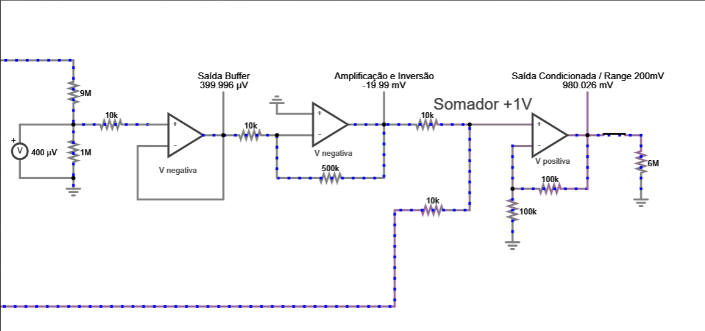
\includegraphics[width=0.8\textwidth]{figuras/cascata.png}
    \fonte{}
\end{figure}

Cada amplificador operacional (amp-op) possui um \textit{drift} de saída, o que introduz ainda mais erro na leitura do \gls{ADC}. Além disso, como é necessária uma amplificação final do sinal, quaisquer ruídos introduzidos também serão amplificados. Com esses problemas combinados, decidiu-se realizar a leitura no modo diferencial, que é a outra opção de leitura nativa disponível no \gls{ADC} escolhido.

\subsubsection{ADC - Modo Diferencial}\label{modo-diferencial}

Este tipo de leitura, ao invés de comparar a tensão entre um ponto do circuito e o \textit{ground}, compara a tensão entre dois pontos do circuito e mede efetivamente a diferença entre elas, como mostrado na \autoref{fig:difread}. Isso significa que nenhuma das entradas está ligada a uma referência, eliminando assim problemas referentes ao isolamento da leitura com o terra e também eliminando ruídos de entrada, pois como estes são introduzidos dos dois lados, eles se cancelam.

\begin{figure}[htb!]
    \caption{Condicionamento de sinais por divisor resistivo para leitura diferencial}
    \label{fig:difread}
    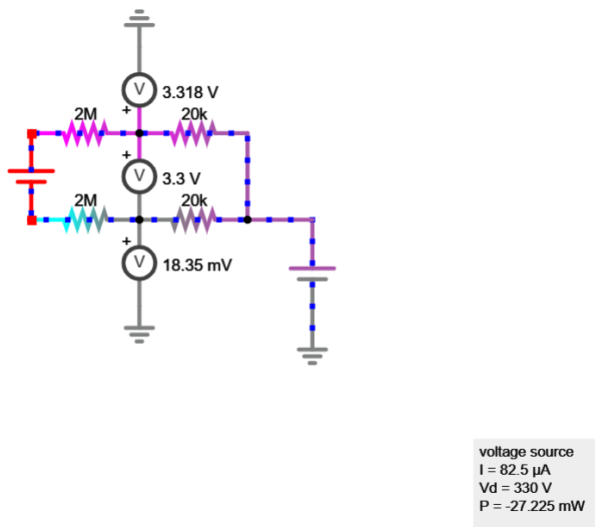
\includegraphics[width=0.6\textwidth]{figuras/difread.png}
    \fonte{}
\end{figure}

Para o dimensionamento dos resistores desta topologia, é necessário atenuar a tensão em aproximadamente 100 vezes, uma vez que um sinal de 330 V (o pico máximo suportado pelo sistema) deve ser condicionado para, no máximo, 3,3 V. Considerando o divisor resistivo, essa atenuação requer uma relação de cerca de 100 vezes entre os resistores. Para garantir uma corrente mínima de entrada, foi escolhido um resistor de 2 M$\Omega$, o que define o segundo valor em 20 k$\Omega$.

Para o offset de tensão, como os erros introduzidos são minimizados pela própria topologia, utiliza-se uma referência de tensão menos precisa, diminuindo o custo do circuito regulador como um todo. A referência de tensão utilizada para este projeto é fornecida pelo \gls{CI} TL431A, tendo este ainda assim uma precisão de 1\%, mas sendo muito mais barato que a opção anterior. Além disso, este possibilita a utilização do range inteiro de leitura do \gls{ADC}, sendo necessário apenas um offset de $3,3/2 V$, utilizado para garantir que as entradas do ADC não recebam tensões negativas, e que pode ser regulado pela ação do \textit{trimpot} junto ao circuito auxiliar. Como não são utilizados \gls{amp-op}s, também não é necessária a utilização do circuito auxiliar \textit{Negative Charge Pump}.

Então, com todos estes benefícios em mente, foi escolhida esta topologia e tipo de leitura para o circuito final, como explícito na \autoref{fig:circ-cond-t}. Para a leitura de corrente, a mesma lógica se aplica, pois o resistor shunt é visto como uma fonte de tensão pelo circuito de leitura. Como esta tensão é extremamente baixa, não há a necessidade de um resistor de entrada para a atenuação da mesma, como explícito na \autoref{fig:circ-cond-c}.

\begin{figure}[htb!]
    \caption{Circuito de condicionamento de sinais para tensão}
    \label{fig:circ-cond-t}
    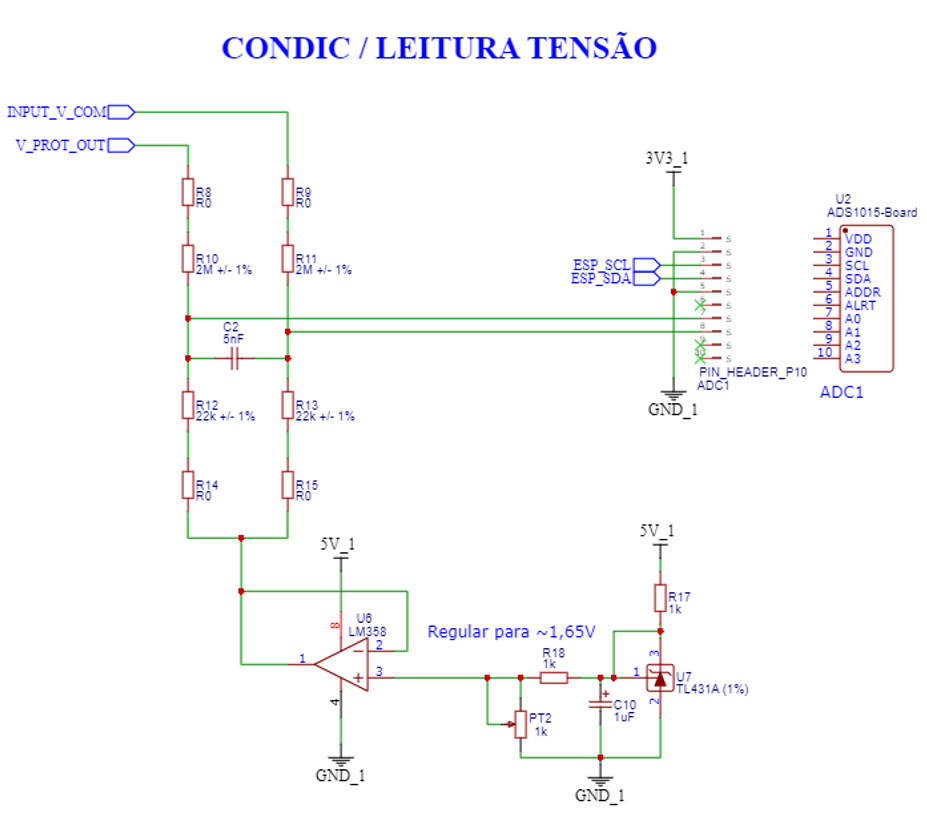
\includegraphics[width=0.8\textwidth]{figuras/circ-cond-t.png}
    \fonte{}
\end{figure}

\begin{figure}[htb!]
    \caption{Circuito de condicionamento de sinais para corrente}
    \label{fig:circ-cond-c}
    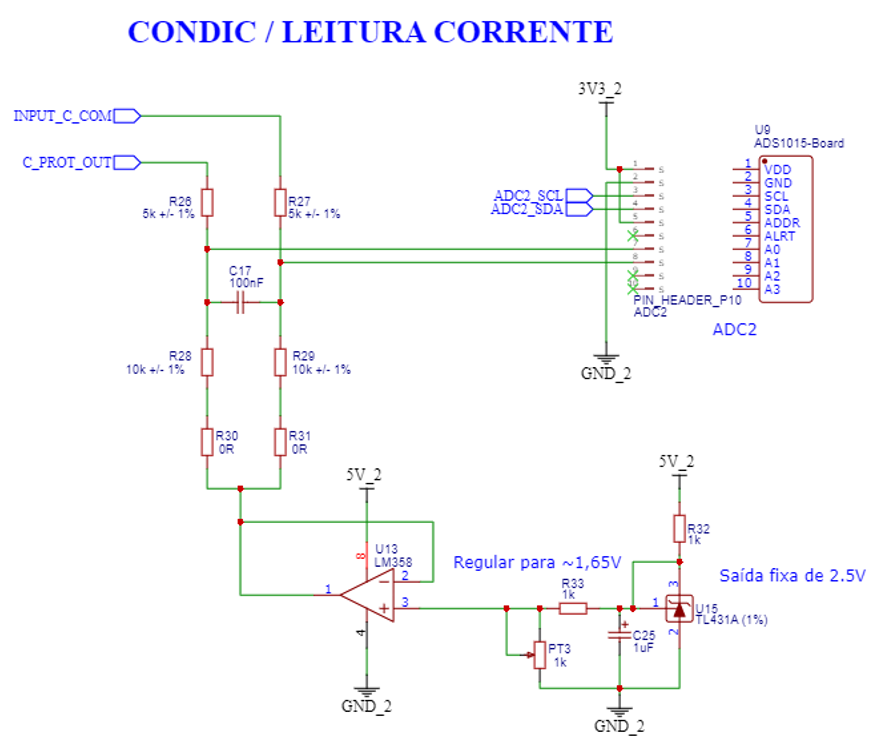
\includegraphics[width=0.8\textwidth]{figuras/circ-cond-c.png}
    \fonte{}
\end{figure}

Também sobre o condicionamento de sinais, é de suma importância se ter um filtro de entrada. Mesmo que a topologia em questão minimize ruídos, quanto mais limpo o sinal de entrada é, melhor serão as leituras e consequentemente o tratamento dos dados. Para este projeto, decidiu-se utilizar um filtro passa-baixas "RC", que consiste de um resistor e um capacitor em \textit{shunt} \cite{filtros}. O cálculo deste filtro é regido pela fórmula \autoref{eqcap}:

\begin{equation}
    \label{eqcap}
    f_{c} = \frac{1}{2\pi RC}
\end{equation}

Este filtro age de forma a atenuar em \textit{3dB} (70,7\%) sinais de frequências maiores que a de corte.

Para o cálculo deste filtro, precisa-se encontrar o R equivalente nos nós do capacitor. Para tanto, utiliza-se o teorema de Thevenin (considerando todas as fontes de corrente como circuito aberto e fontes de tensão como curto), como é possível verificar substituindo o capacitor por um ohmímetro na \autoref{fig:r-thevenin}.

\begin{figure}[htb!]
    \caption{Simulação da resistência de Thevenin}
    \label{fig:r-thevenin}
    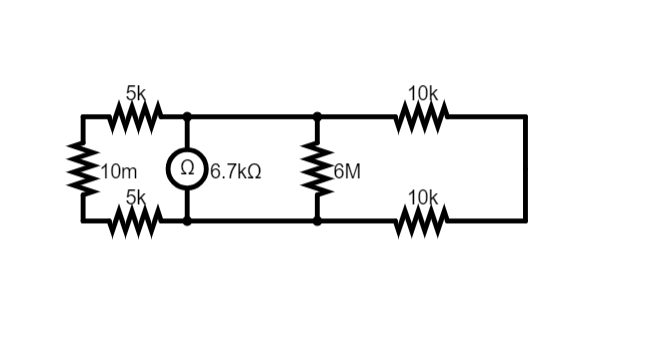
\includegraphics[width=0.9\textwidth]{figuras/r-thevenin.png}
    \fonte{}
\end{figure}

Utilizando a fórmula, para o caso da entrada de corrente e considerando dois resistores de 5 k$\Omega$ (pela facilidade de se encontrar o componente), chega-se ao valor de um capacitor de aproximadamente 100 nF para uma frequência de corte de aproximadamente 237 \textit{Hz}. As simulações representadas nas figuras \ref{fig:simco1} e \ref{fig:simco2}. O sinal encontrado no resistor de 6 M$\Omega$ representa a entrada do \gls{ADC}.

\begin{figure}[htb!]
    \caption{Simulação sem filtro passa-baixa para a corrente}
    \label{fig:simco1}
    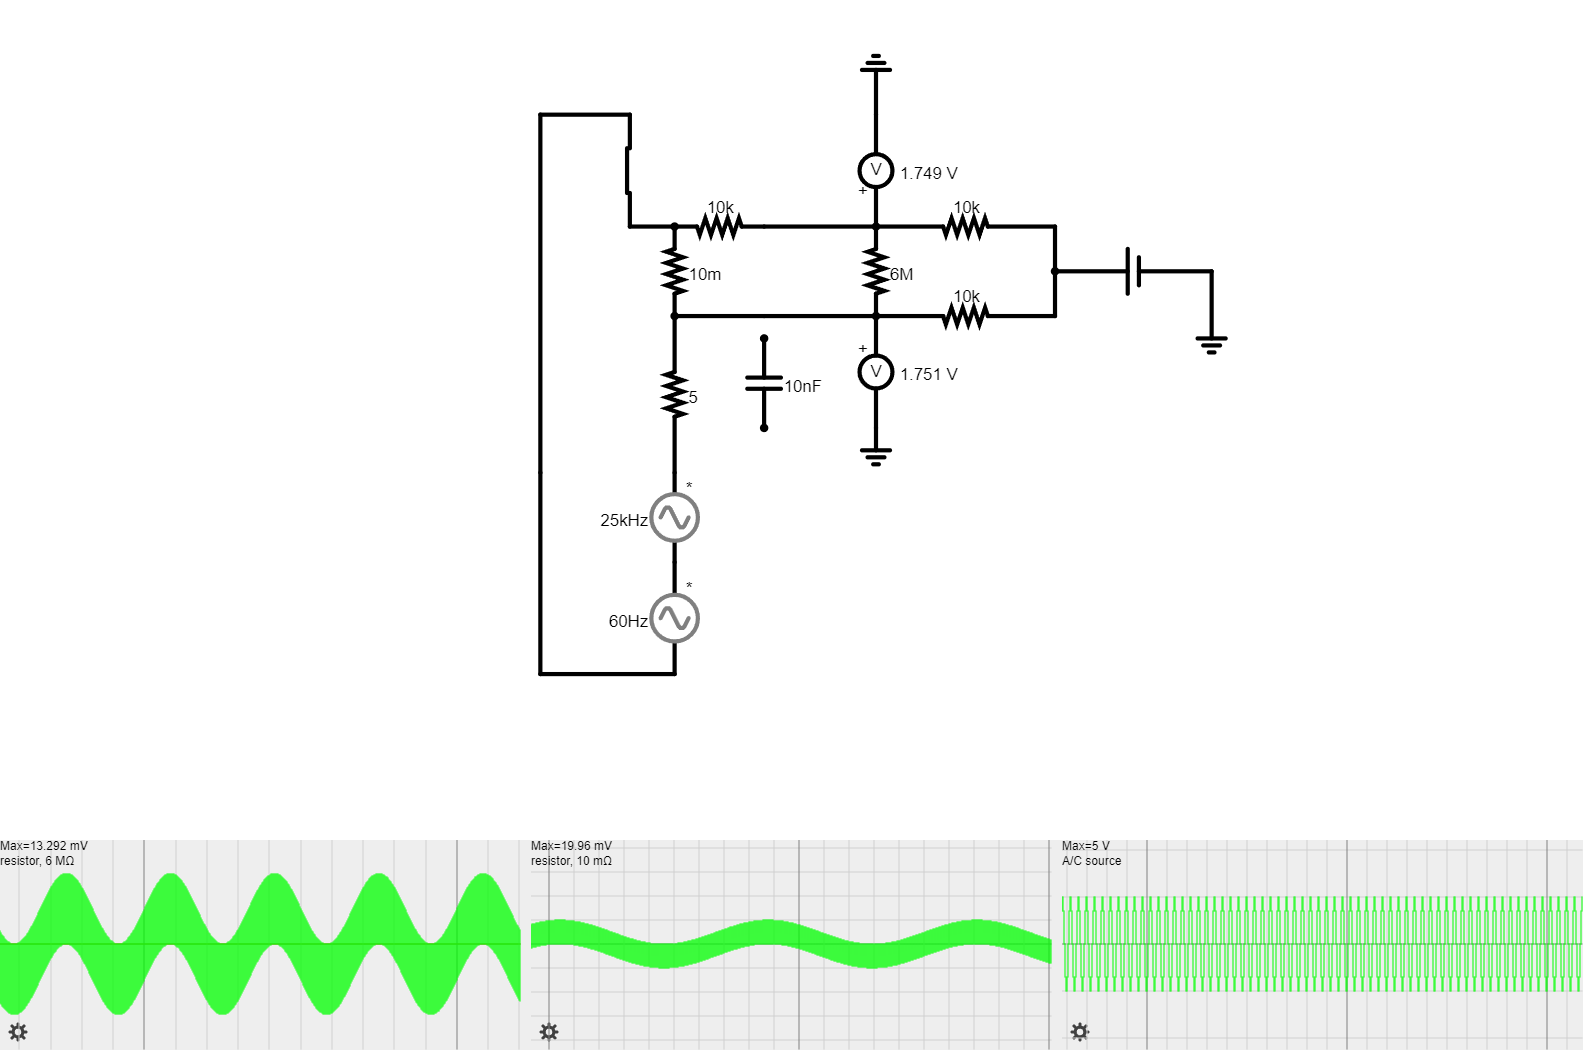
\includegraphics[width=0.9\textwidth]{figuras/sim-co-1.png}
    \fonte{}
\end{figure}

\begin{figure}[htb!]
    \caption{Simulação com filtro passa-baixa para a corrente}
    \label{fig:simco2}
    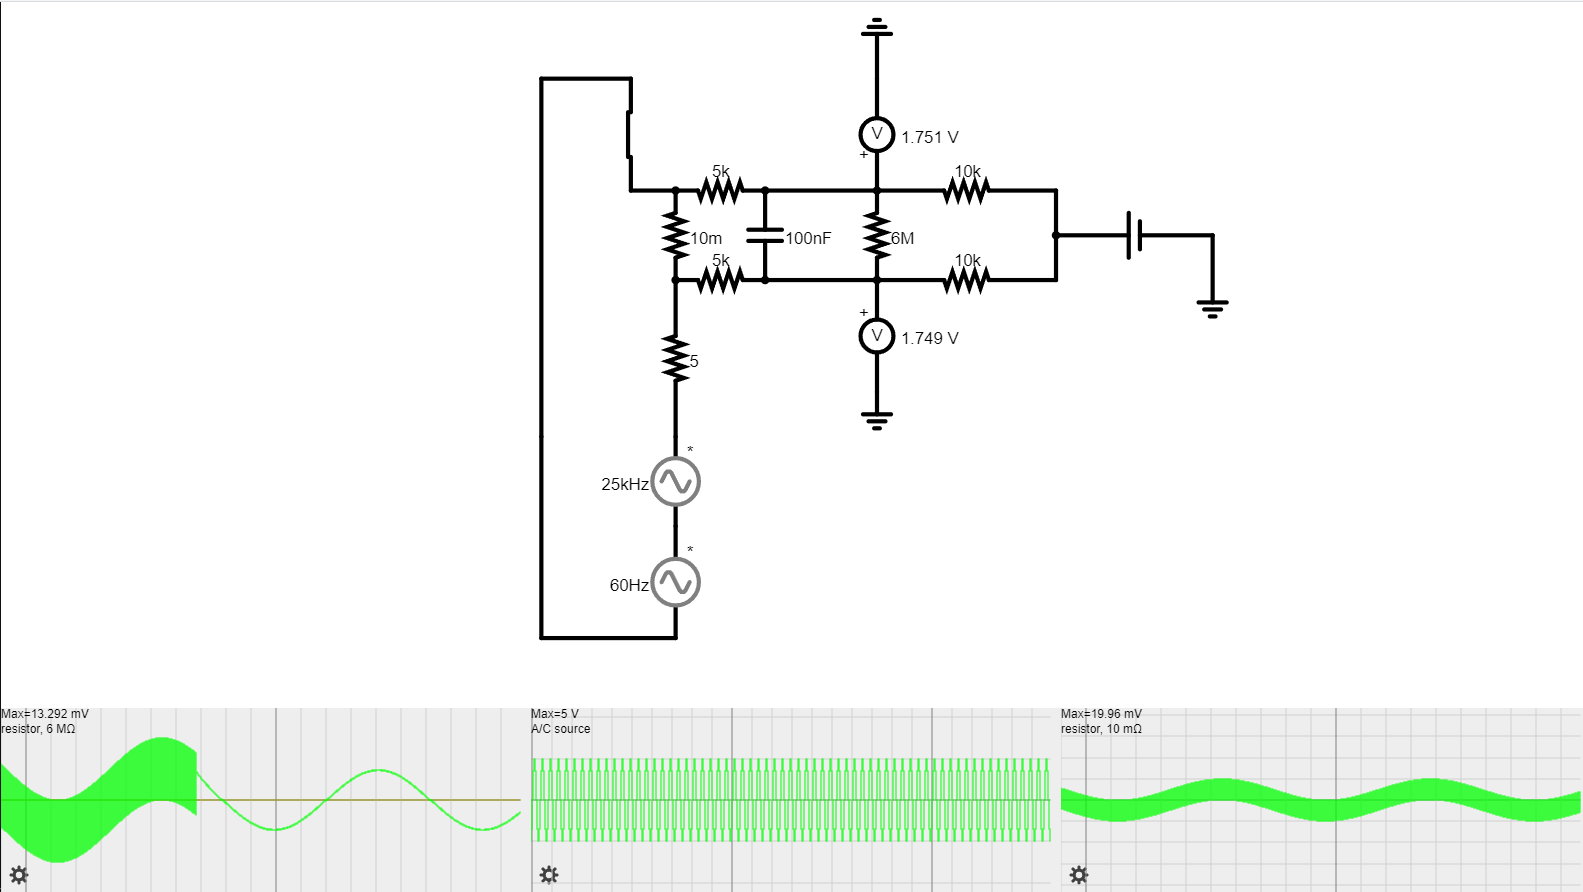
\includegraphics[width=0.9\textwidth]{figuras/sim-co-2.png}
    \fonte{}
\end{figure}

Para a entrada de tensão do circuito segue-se a mesma lógica, chegando a um valor de aproximadamente 5 nF.

Após a leitura dos sinais e a conversão feita pelo ADC, o sinal digital de saída é processado por um microcontrolador para então ser entregue a uma webpage e assim tratado para visualização pelo usuário. 

\subsubsection{Isolamento}\label{isolamento-metodologia}

Para que a leitura diferencial ocorra de maneira adequada, é necessário que haja um caminho de retorno para os sinais medidos - uma vez que a medição ocorre aferindo a tensão de cada uma das entradas do \gls{ADC} em relação a referência e diferenciando-as \cite{mediff}.
Essa referência pode ser obtida de maneira direta, utilizando uma conexão separada com a função específica de se tornar o caminho para os sinais de tensão e corrente, representada na \autoref{fig:diff-3-wire}. Ou pode ser obtida de maneira indireta, conectando internamente uma das ponteiras do dispositivo também ao \textit{GND} (ou ponto comum) do \gls{ADC}, fazendo com que não seja necessário o uso de um fio dedicado para esse fim, conforme a \autoref{fig:diff-2-wire}.

\begin{figure}[htb!]
    \caption{Circuito diferencial simplificado com conexão específica para referência}
    \label{fig:diff-3-wire}
    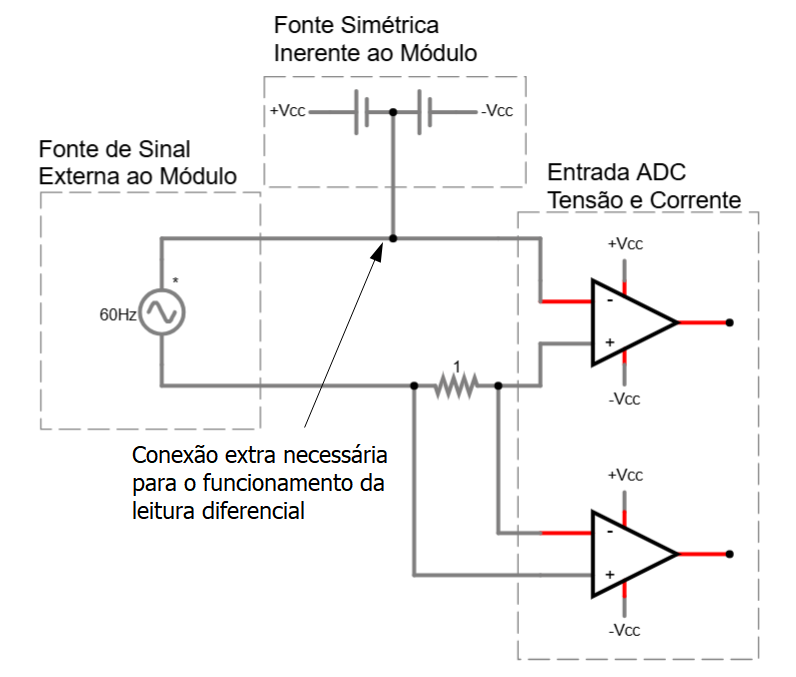
\includegraphics[width=0.7\textwidth]{figuras/diferencial-3-fios.png}
    \fonte{}
\end{figure}

\begin{figure}[htb!]
    \caption{Circuito diferencial simplificado sem conexões adicionais}
    \label{fig:diff-2-wire}
    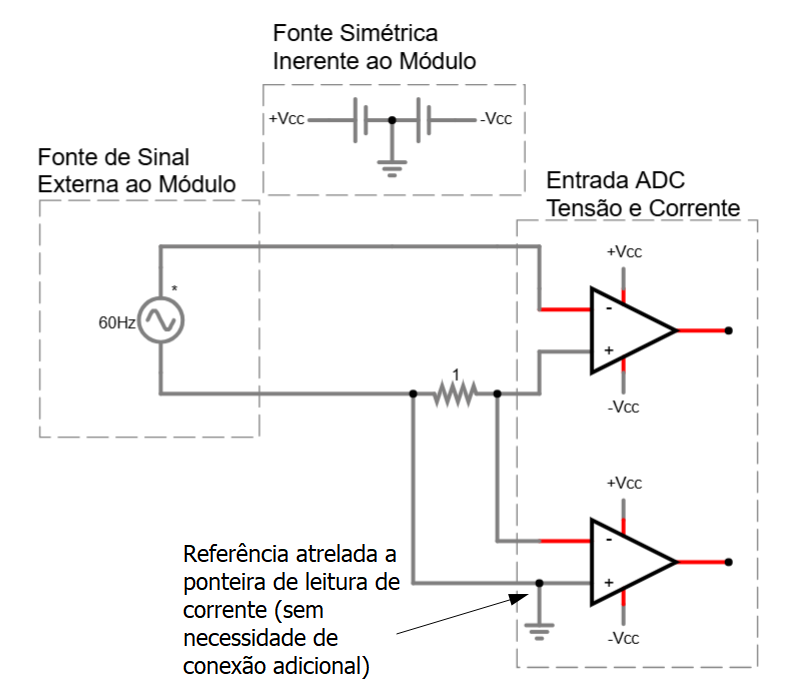
\includegraphics[width=0.7\textwidth]{figuras/diferencial-2-fios.png}
    \fonte{}
\end{figure}

Ambas as propostas são funcionais e aplicáveis, porém, devido a especifidades de cada uma, foram descartadas para esse projeto. A leitura feita com a conexão auxiliar implica na necessidade de um uso não convencional e pouco realista do cotidiano do laboratório onde as matérias alvo desse trabalho serão ministradas. Já a topologia que não possui conexões adicionais tornaria a leitura de somente uma grandeza por vez (tensão ou corrente) impossibilitada, dependendo de qual ponto foi escolhido para estar atrelado a referência interna.

Uma vez que não é adequado referenciar o circuito em mais de um ponto, devido a possibilidade de curto-circuitos indesejados conforme a conexão das ponteiras feita pelo usuário, como exemplo a \autoref{fig:curto-diferencial}. Propôs-se o isolamento de cada canal, utilizando fontes internas isoladas.

\begin{figure}[htb!]
    \caption{Circuito diferencial simplificado com referência em mais de uma ponteira}
    \label{fig:curto-diferencial}
    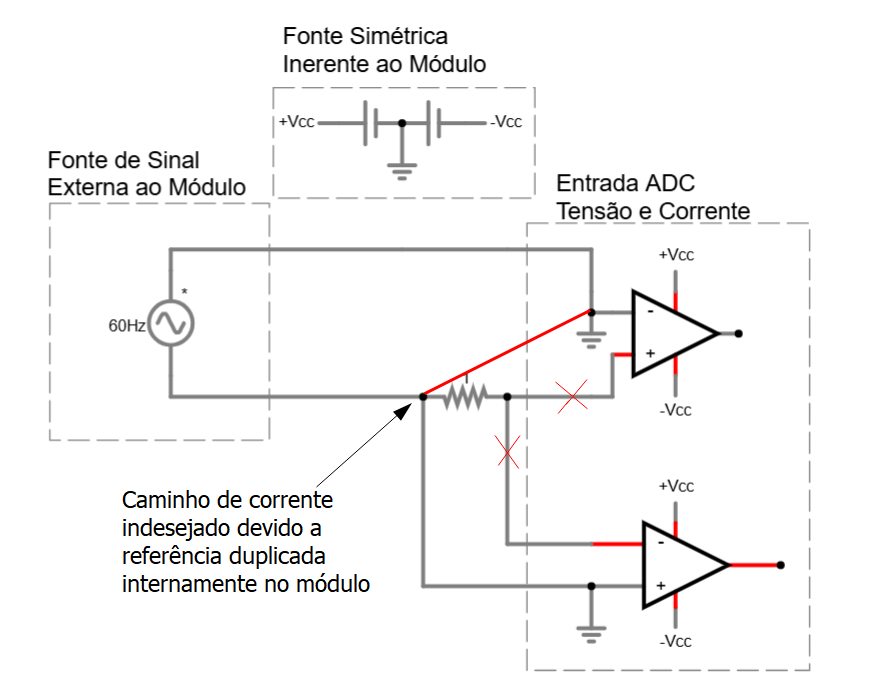
\includegraphics[width=0.7\textwidth]{figuras/diferencial-em-curto.png}
    \fonte{}
\end{figure}

Dessa maneira, é possível ter a referência de tensão diretamente na ponteira de leitura para cada um dos canais, sem que haja a possibilidade de curto-circuito e, como consequência indireta da topologia, ainda diminui interferências que as leituras poderiam causar entre si. Essa topologia pode ser melhor visualizada através da \autoref{fig:dif-isolado}.
Conforme comentado na \autoref{subsec:protecaoTensao}, uma outra alternativa seria a utilização de amplificadores operacionais isolados, porém esses apresentam preço extremamente elevado para o escopo do trabalho, sendo essa alternativa descartada.

\begin{figure}[htb!]
    \caption{Circuito diferencial simplificado isolado}
    \label{fig:dif-isolado}
    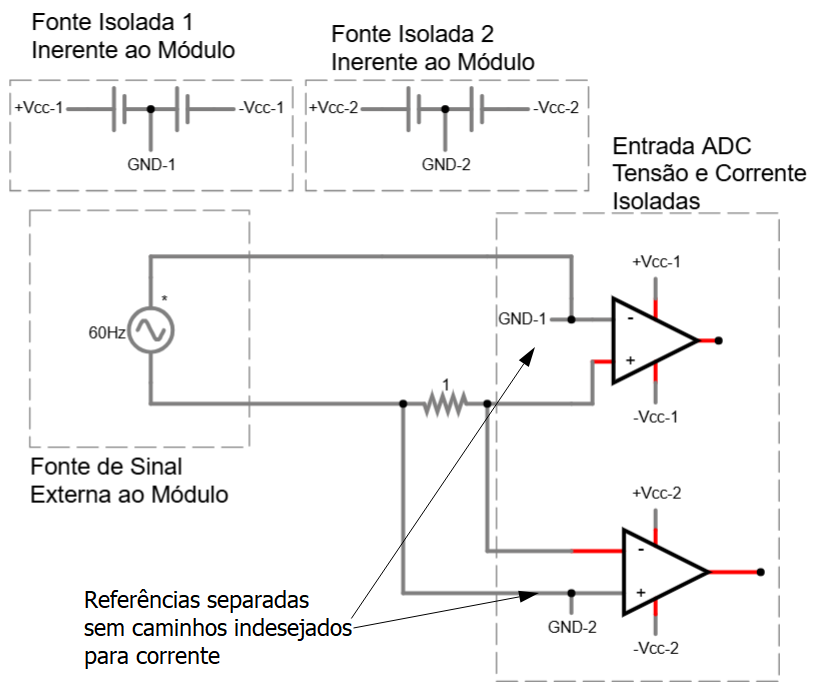
\includegraphics[width=0.7\textwidth]{figuras/diferencial-ref-separada.png}
    \fonte{}
\end{figure}

Para se ter uma comunicação confiável entre os dois \gls{ADC}s conectados a fontes diferentes e o ESP32, é necessário o isolamento dos sinais utilizados para a comunicação. Para isso, foi utilizado um circuito isolado por \textit{optocouplers}, como demonstrado na \autoref{fig:circ-comunic}.

\begin{figure}[htb!]
    \caption{Circuito de comunicação isolado}
    \label{fig:circ-comunic}
    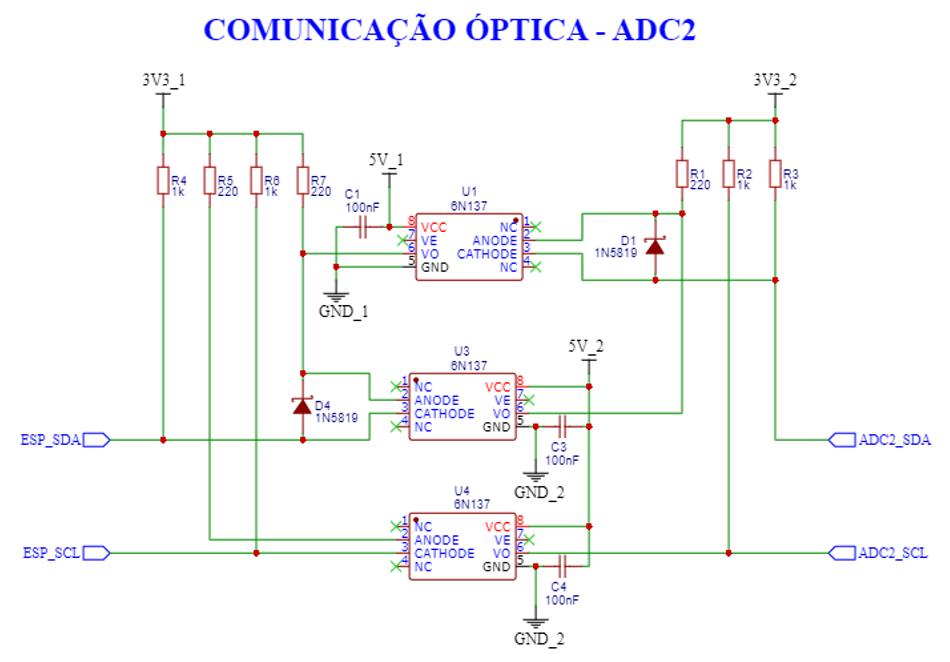
\includegraphics[width=1.0\textwidth]{figuras/circ-comunic.png}
    \fonte{}
\end{figure}

O circuito transforma pulsos \gls{$I^2$C} em sinais de luz e transfere estas informações para o outro circuito isolado, desacoplando estes. Para o correto funcionamento do circuito, devido a limitações técnicas dos \textit{optocouplers} escolhidos, é necessária a inserção de uma linha de 5 V para a alimentação do \gls{CI}, bem como o uso de uma linha de 3,3 V para a ativação dos LEDs internos deste chip, bem como o potencial de \textit{pull-up} para as linhas de comunicação \gls{$I^2$C}.

\subsubsection{Modularidade no Hardware}\label{modularidade-metodologia}

Um dos principais objetivos da proposta desenvolvida foi possibilitar a leitura simultânea de duas ou três fases diferentes. Para tanto, o dispositivo precisaria operar com quatro ou seis canais isolados entre si, devido às implicações supracitadas. Essa configuração elevaria o custo, o espaço físico e a complexidade de apenas um dispositivo, sendo que, em diversas etapas das disciplinas de circuitos, apenas a leitura de uma das fases é utilizada – considerando-se o circuito trifásico equilibrado.

Optou-se, então, por tornar o dispositivo modular. Dessa forma, cada módulo é composto por um medidor de tensão e corrente isoladas, e, caso haja a necessidade de expansão, basta adicionar módulos extras e interconectá-los, de modo que comuniquem entre si e enviem os dados lidos.

Assim, um módulo principal coordena as leituras dos módulos secundários, recebe os dados por meio de algum protocolo de comunicação e envia os valores obtidos para a interface homem-máquina, conforme ilustrado no diagrama da \autoref{fig:modularidade-fisica}.

\begin{figure}[htb!]
    \caption{Diagrama de conexão modular entre dispositivos}
    \label{fig:modularidade-fisica}
    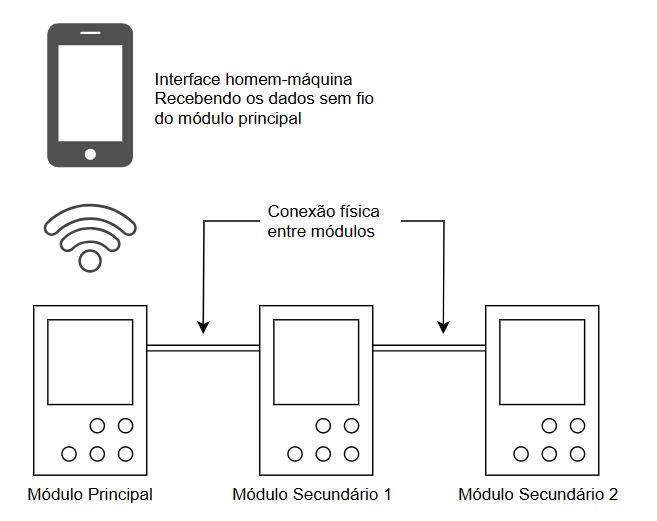
\includegraphics[width=0.8\textwidth]{figuras/mod-fisica.png}
    \fonte{}
\end{figure}

Inicialmente, considerou-se o uso do protocolo \gls{$I^2$C} para a comunicação entre os módulos. No entanto, essa abordagem foi descartada devido à complexidade de criação de um protocolo ou dicionário que estabelecesse um modo comum de interação. Esse protocolo seria implementado fisicamente da mesma forma proposta para a comunicação isolada entre o ESP32 e o \gls{ADC} (que não compartilham a mesma referência), utilizando optoacopladores, conforme ilustrado na \autoref{fig:circ-comunic}.

Diante dessas considerações, concluiu-se que a utilização do protocolo \textit{ESP-NOW} – desenvolvido pela Espressif para facilitar a comunicação entre chips que possuem \textit{WiFi} – em conjunto com o protocolo de comunicação via \textit{websockets}, já utilizado para a comunicação entre o dispositivo e a interface homem-máquina, seria mais adequada para este caso. Dessa forma, os dados dos dispositivos secundários são transferidos de forma sem fio para o dispositivo principal.

Como as leituras dos dispositivos são sensíveis a atrasos, devido à natureza das medições no tempo, é necessária uma conexão física entre os módulos para sincronizar as leituras. Assim, o dispositivo principal envia aos demais módulos um pulso indicando o início de uma nova série de dados, permitindo que todos realizem a amostragem dentro da mesma janela temporal. Dessa maneira, são necessários apenas dois fios conectando cada dispositivo, sendo estes a saída do sinal isolado, transmitido por meio de um optoacoplador, conforme ilustrado na \autoref{fig:modular-sinc}.

\begin{figure}[htb!]
    \caption{Detalhe da conexão modular entre dispositivos utilizando dois fios para sincronização de leituras}
    \label{fig:modular-sinc}
    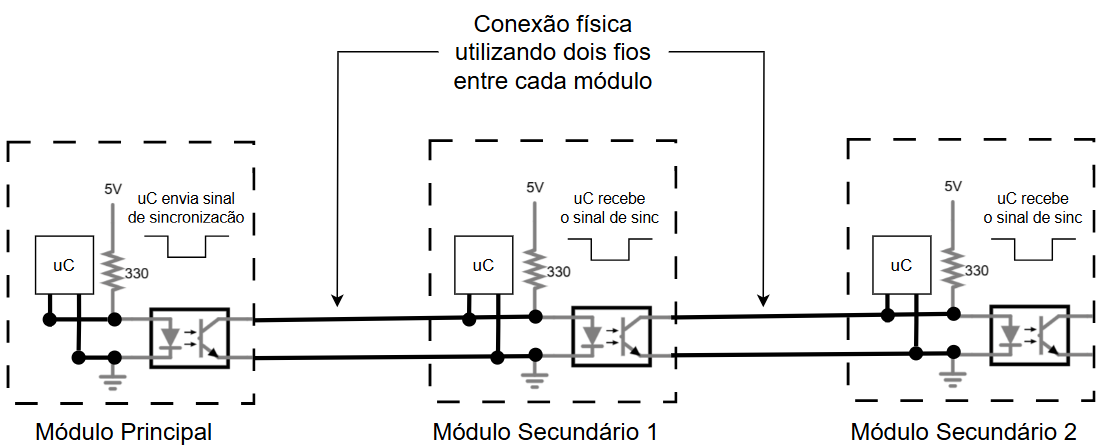
\includegraphics[width=1.0\textwidth]{figuras/mod-fisica-detalhe.png}
    \fonte{}
\end{figure}

Este circuito adicional, no entanto, não foi implementado no presente trabalho devido a dificuldades encontradas durante o desenvolvimento, conforme descrito na \autoref{dificuldades-futuro}. Sugere-se, portanto, que futuras melhorias neste estudo considerem a aplicação desse circuito, dado seu potencial para expandir o sistema.

\subsubsection{Microcontrolador}\label{uC-metodologia}

Algumas necessidades básicas devem ser atendidas pelo chip escolhido, como suporte para comunicação \textit{wireless}, seja \textit{WiFi} ou \textit{Bluetooth}, \textit{clock speed} alta o suficiente para não interferir na aquisição de dados e também ter uma boa documentação para ser possível o desenvolvimento do código.

Portanto, o microcontrolador utilizado para este projeto é o ESP32, fabricado pela Espressif. A escolha deste foi feita por vários motivos:

\begin{itemize}
    \item Performance: O ESP32 opera em \textit{clock speeds} de até 240 MHz, oferecendo um robusto poder de processamento para o código e também para não interferir ou atrasar a aquisição dos sinais;
    \item Suporte: Este microcontrolador tem suporte tanto para \textit{WiFi} quanto para \textit{Bluetooth}, trabalha com o protocolo \gls{$I^2$C}, que será utilizado para fazer a comunicação com o \gls{ADC} e utiliza-se do Arduino como sua principal plataforma de desenvolvimento;
    \item Ambiente: Este módulo é extensamente utilizado em vários setores da tecnologia e tem uma vasta comunidade de usuários, o que garante um extenso leque de \textit{resources} como bibliotecas, tutoriais, videos, forums, entre outros, para ajudar na confecção do software e firmware. Também apresenta suporte oferecido pela própria Espressif sobre as suas funcionalidades muito bem documentados;
    \item Modularidade: Esta parte do trabalho também é facilitada devido ao componente já possuir nativamente protocolos de comunicação da própria fabricante;
    \item Preço: Para todas as funcionalidades providas pelo ESP32, este apresenta um grande custo benefício, além de estar facilmente disponível no mercado.
\end{itemize}

\subsubsection{Alimentação e regulação de tensão}

Para a alimentação dos circuitos integrantes do protótipo, existem duas opções: baterias ou fontes. Como este será utilizado em bancada, foi escolhida a alimentação por fontes, pois estas não precisam ser trocadas frequentemente e é possível ligá-las à rede, além de algumas outras vantagens.

Neste projeto são utilizadas duas fontes isoladas galvanicamente, uma para alimentar o circuito de leitura de tensão e outra para alimentar o circuito de leitura de corrente, reduzindo ainda mais possíveis ruídos e interferências entre circuitos, mas também aumentando a confiabilidade do protótipo, pois como o objetivo é realizar leituras simultâneas de corrente e tensão, o isolamento entre eles é necessário para prevenir curtos.

Porém, o saída das fontes escolhidas é de 12 V, não atendendo as necessidades de alimentação dos \gls{CI}s envolvidos e também do microcontrolador. Para isso, circuitos de regulação de tensão foram implementados, gerando duas saídas, como explícito na \autoref{fig:circ-conv-T}. Estes circuitos são iguais tanto para a leitura de tensão e de corrente, visto que estes tem as mesmas necessidades.

\begin{figure}[htb!]
    \caption{Circuito de regulação de tensão}
    \label{fig:circ-conv-T}
    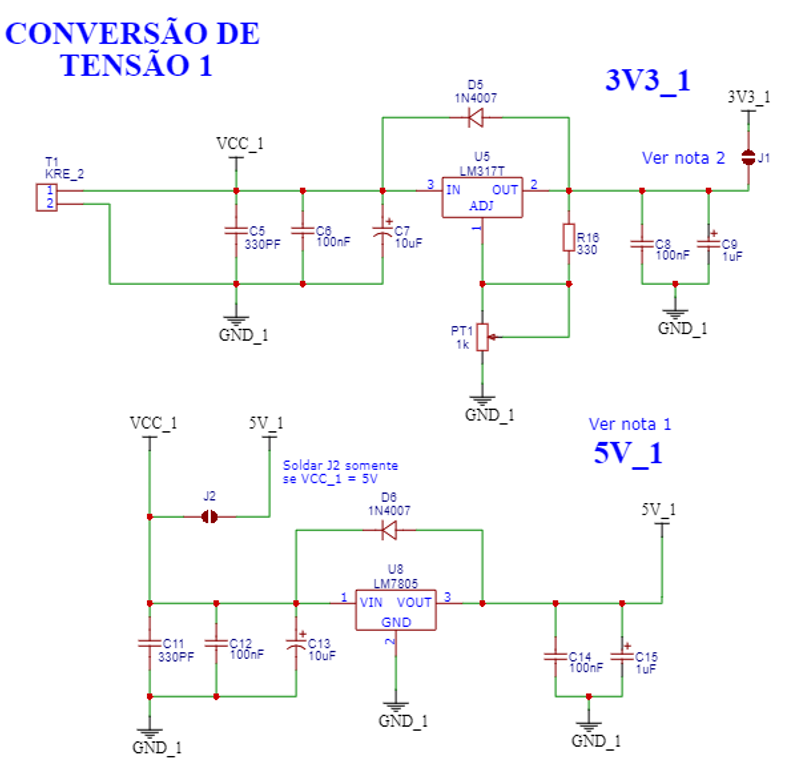
\includegraphics[width=0.8\textwidth]{figuras/circ-conv-T.png}
    \fonte{}
\end{figure}

A alimentação do ESP32 e também do circuito de comunicação isolada foi definida como 5 V por especificação de projeto, para manter um padrão e também suprir as necessidades de cada.

\subsubsection{Disponibilidade do Circuito}\label{availability}

O circuito pode ser encontrado na integra no [APENDICE X -TODO-] ao final do trabalho, bem como de maneira virtual no mesmo anexo. Dada a característica colaborativa da plataforma em que foi desenvolvido, permite que qualquer usuário clone esse circuito e o modifique gratuitamente.

\subsection{Software e Firmware}\label{softfirm}

A programação do dispositivo é separada em duas etapas: \textit{Firmware} e \textit{Software}. O \textit{Firmware} é responsável por garantir a funcionalidade da comunicação do microcontrolador com os módulos \gls{ADC}, bem como manter a comunicação sem fio e sincronizar a amostragem do sinal.
Já o \textit{Software}, é responsável por receber as entradas do usuário e mostrar, efetivamente, através de gráficos e valores numéricos, as leituras de tensão, corrente, frequência, potências, etc.
Outra parte importante da programação trata-se da modularidade. Essa está presente tanto no \textit{Firmware} quanto no \textit{Software}. Trata-se da possibilidade de utilizar mais de um dispositivo em conjunto com um principal, permitindo a leitura de mais fases de maneira isolada.

\subsubsection{Firmware}\label{firmw}

O \textit{Firmware} é a parte crítica que roda diretamente no microcontrolador ESP32 e é responsável pela interface com os sensores, controle de comunicação sem fio e envio dos dados coletados para o \textit{Software} via WebSockets. Ele também gerencia a sincronização das leituras do ADC, garantindo que os dados de tensão e corrente sejam capturados e processados de forma precisa.

O desenvolvimento do \textit{Firmware} foi baseado em bibliotecas otimizadas para o ESP32, como a \textit{ESPAsyncWebServer} e a \textit{WebSocketsServer}, que permitem uma comunicação eficiente com o dispositivo remoto (celular ou computador). Além disso, foi utilizada a biblioteca \textit{ADS1015\_WE} para interface com o ADC externo ADS1015, permitindo leituras de alta precisão de sinais analógicos.

A sincronização entre os sinais de tensão e corrente é feita por meio de interrupções, que detectam o momento em que os dados estão prontos para leitura. Isso garante que as amostragens estejam alinhadas e que os gráficos e cálculos de potência sejam precisos. Para garantir a modularidade do sistema, o \textit{Firmware} também possui a capacidade de alterar a faixa de leitura da tensão e da corrente dinamicamente, de acordo com o comando enviado pelo usuário via WebSockets.

Uma parte importante do \textit{Firmware} é a implementação da máquina de estados, mostrada na \autoref{fig:maq-estado-simp}, que gerencia a comunicação com o dispositivo auxiliar (interface homem-máquina). A implementação foi feita para ser expansível, permitindo a futura integração de múltiplos dispositivos sem a necessidade de grandes modificações no código.

\begin{figure}[htb!]
    \caption{Máquina de estados simplificada para apenas um dispositivo}
    \label{fig:maq-estado-simp}
    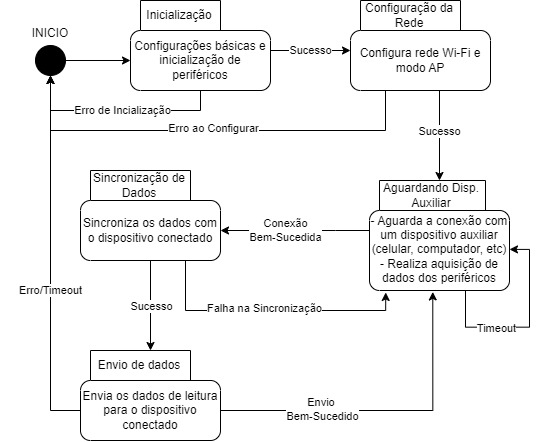
\includegraphics[width=1.0\textwidth]{figuras/Maquina-Estados-Simplificada.jpg}
    \fonte{}
\end{figure}

O processo de comunicação sem fio utiliza o protocolo \textit{WiFi} integrado do ESP32 para criar um ponto de acesso, facilitando a interação com o dispositivo móvel. O firmware também é responsável por lidar com a detecção de conexões e desconexões dos clientes WebSocket, ajustando o comportamento do sistema conforme necessário.

Seguindo a lógica proposta, o microcontrolador, ao ser energizado, completa sua rotina de \textit{setup} e permanece disponível para conexões. Após o estabelecimento da conexão, configura-se a relação principal entre o servidor, como \textit{master}, e o dispositivo conectado, como \textit{main client}. Ao acessar o IP do ESP32, ele serve à \textit{webpage} o HTML e JavaScript necessários para sua apresentação e interação.

Quando a leitura é iniciada, o microcontrolador executa todas as etapas necessárias, incluindo o envio do pulso de \textit{sync} (sincronização) e a criação de um delta de tempo para estabelecer um ponto de referência zero. Este último possibilita a sincronização das ondas, além do cálculo da frequência e do fator de potência. A aquisição dos dados em si também envolve uma série de processos específicos.

O \gls{ADC}, acompanhado pelo circuito de condicionamento de sinais, pode operar em dois modos de leitura: \textit{Data-Ready} e \textit{Single-Shot}.

No modo \textit{Single-Shot}, o processador solicita as leituras ao \gls{ADC}, que processa e envia os dados requisitados. Embora esse modo seja simples de implementar e bastante confiável, as limitações do chip escolhido tornam essa solução lenta para a aplicação em questão, alcançando uma taxa máxima de leitura de cerca de 500 \gls{SPS}, insuficiente para a aquisição desejada da forma de onda.

Optou-se, então, pelo modo \textit{Data-Ready}, que é mais complexo. Porém, nesse modo, após cada leitura, o \gls{ADC} sinaliza ao microcontrolador levantando uma \textit{flag} (por exemplo, elevando um pino específico para \textit{high}) indicando que os dados estão prontos, aguardando a ação do processador. Quando o processador requisita os dados, eles são removidos do \textit{cache} do \gls{ADC}, reiniciando o ciclo de leitura. Com esse método, foi possível atingir uma taxa de 3300 \gls{SPS}, permitindo uma aquisição mais precisa da forma de onda.

Os valores adquiridos pelo \gls{ADC} são então processados pelo ESP32 para converterem-se em valores reais. Esse processamento começa com a seleção de uma faixa de leitura (\textit{range}) via o \textit{Programmable-gain Amplifier} (\gls{PGA}).

Uma vez processados, os dados puros são armazenados em uma \textit{struct}, conforme a estrutura da \autoref{tab:struct-graph}, serializados em formato JSON e enviados à \textit{webpage} para visualização. Caso não haja novas entradas do cliente, esse processo se repete indefinidamente.

\begin{table}[h!]
\centering
\caption{Chart data}
\begin{tabular}{|c|c|c|}
    \hline
    \textbf{Tipo} & \textbf{Nome da Variável} & \textbf{Descrição} \\ \hline
    int8\_t & chart\_id & Identificação do gráfico (usada somente para modularidade) \\ \hline
    int8\_t & voltage\_gain & Ganho de tensão a ser informado para o WebServer \\ \hline
    int8\_t & current\_type & Ganho/faixa de corrente a ser informada para o WebServer (mA, A, uA) \\ \hline
    int16\_t & voltage\_value[ ] & Array de valores das tensões lidas \\ \hline
    int16\_t & current\_value[ ] & Array de valores das correntes lidas \\ \hline
    int64\_t & voltage\_time[ ] & Array de valores dos tempos em que cada tensão foi lida \\ \hline
    int64\_t & current\_time[ ] & Array de valores dos tempos em que cada corrente foi lida \\ \hline
\end{tabular}
\label{tab:struct-graph}
\end{table}

\subsubsection{Software}\label{softwa}

Toda a lógica de conversão dos valores de tensão e corrente em bits do \gls{ADC} para os valores reais é feita através de javascript em uma webpage. Dessa maneira, poupa-se informação transmitida pelo módulo, e utiliza-se um processamento mais robusto (do celular ou computador conectado) para os cálculos de potência.

Esta webpage foi desenvolvida em HTML5 com integração de JavaScript e uso do protocolo WebSocket. Esse protocolo permite uma conexão bidirecional entre o servidor do microcontrolador e o dispositivo móvel. A interface processa os dados e os apresenta ao usuário por meio de gráficos e indicadores numéricos. São exibidos valores de tensão RMS, corrente RMS, frequência, potências (aparente, reativa e ativa) e Fator de Potência.

\subsubsubsection{Tensão e Corrente}
Para diferentes configurações de escala de tensão, o código utiliza multiplicadores pré-definidos para converter os valores lidos para a tensão real. A \autoref{tab:softw-tensao} descreve os multiplicadores e a escala máxima correspondente:

\begin{table}[h!]
    \centering
    \caption{Tabela de multiplicadores de tensão}
    \begin{tabular}{|c|c|c|c|}
        \hline
        \textbf{Multiplicador} & \textbf{Tensão Máxima na Escala (V)} & \textbf{Ganho} & \textbf{Tensão Máxima (V)} \\
        \hline
        0.2 & 409.6 & 1 & 4.096 \\
        0.1 & 204.8 & 2 & 2.048 \\
        0.05 & 102.4 & 4 & 1.024 \\
        0.025 & 51.2 & 8 & 0.512 \\
        0.0125 & 25.6 & 16 & 0.256 \\
        \hline
    \end{tabular}
    \label{tab:softw-tensao}
\end{table}

Os valores foram obtidos analisando o circuito, de maneira a sempre manter a tensão na leitura abaixo dos 3.3V de tensão suportados pelo \gls{ADC}. Estes devem ser ajustados conforme a necessidade de calibração do dispositivo montado.

De maneira similar, o mesmo ocorre com a corrente. Porém, devido a aspectos construtivos do módulo, essa sempre está com o \gls{PGA} na escala \textit{x16}, alterando apenas os multiplicadores conforme a \autoref{tab:softw-corrente}.
Os ajustes para cada escala tratam-se dos valores de calibração que devem ser alterados conforme a necessidade após ter o dispositivo físico montado.

% Tabela de multiplicadores de corrente
\begin{table}[h!]
    \centering
    \caption{Tabela de multiplicadores de corrente}
    \begin{tabular}{|c|c|}
        \hline
        \textbf{Escala} & \textbf{Multiplicador} \\
        \hline
        A & $0.01875 \times \text{ajuste\_A}$ \\
        mA & $0.0001856 \times \text{ajuste\_mA}$ \\
        uA & $0.000001875 \times \text{ajuste\_uA}$ \\
        \hline
    \end{tabular}
    \label{tab:softw-corrente}
\end{table}

Os valores dos multiplicadores de corrente foram obtidos analisando o comportamento do circuito e fazendo as devidas conversões de tensão para corrente conforme o valor dos resistores utilizados em cada caso, veja \autoref{tab:softw-corrente-values}:

\begin{table}[h!]
    \centering
    \caption{Tabela de multiplicadores de corrente}
    \begin{tabularx}{\textwidth}{|X|X|X|X|X|X|X|}
        \hline
        \textbf{Range} & \textbf{Resistor shunt} & \textbf{Corrente (A)} & \textbf{Mult. do divisor resistivo} & \textbf{Tensão lida (V)} & \textbf{Mult. inicial (0,125mV/bit)} & \textbf{Mult. final (razão do resistor)} \\
        \hline
        uA & 100 & 0,001 & 1,5 & 0,1000 & 0,0001875 & 0,000001875 \\
        mA & 1,01 & 0,2 & 1,5 & 0,2020 & 0,0001875 & 0,000185644 \\
        A & 0,01 & 10 & 1,5 & 0,1000 & 0,0001875 & 0,018750 \\
        \hline
    \end{tabularx}
    \label{tab:softw-corrente-values}
\end{table}

\subsubsubsection{Apresentação Visual}

Os gráficos são gerados por uma biblioteca do JavaScript chamada Graph.js. Esta biblioteca possibilita a integração de vários gráficos, para a amostragem e apresentação tanto da tensão quanto da corrente simultaneamente, e também a utilização de um \textit{trigger} por programação, para ser possível a visualização da onda estabilizada. Este trigger funciona de forma a detectar a passagem da onda por um ponto escolhido e então sincronizar o gráfico de acordo, tornando aquele o ponto 0 visualizado e então estabilizando a onda.

A parte estrutural da página foi desenvolvida utilizando \gls{HTML}. Exemplos das telas durante a leitura podem ser vistos na \autoref{fig:webpage1} e \autoref{fig:webpage2}.

\begin{figure}[h!]
    \centering
    \caption{Detalhe do cabeçalho de informações da página da Web gerada pelo dispositivo}
    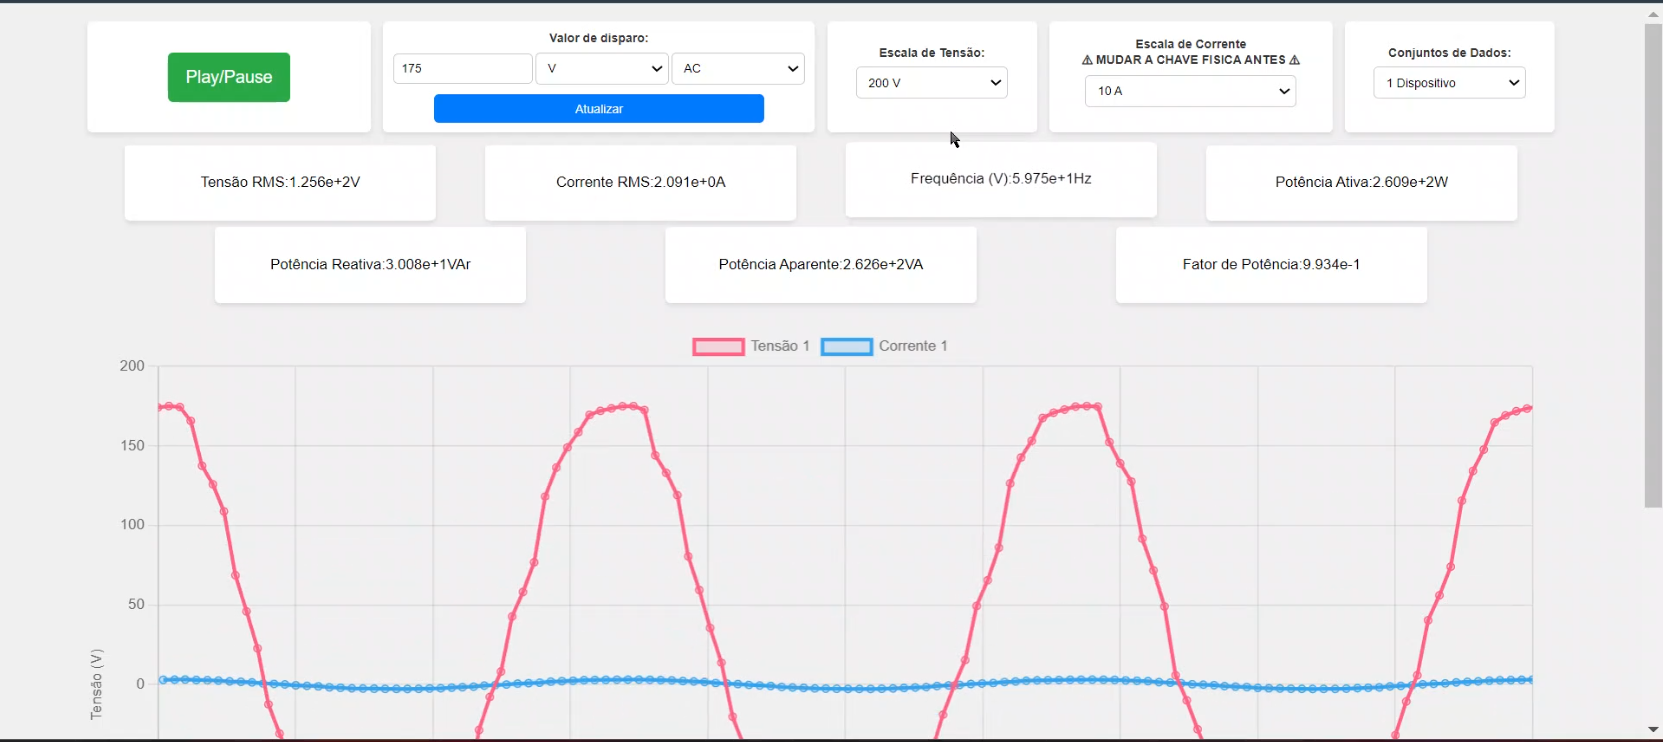
\includegraphics[width=\textwidth, height=\textheight, keepaspectratio]{webpage-tela1.png}
    \label{fig:webpage1}
    \fonte{}
\end{figure}

\begin{figure}[h!]
    \centering
    \caption{Detalhe do gráfico da página da Web gerada pelo dispositivo}
    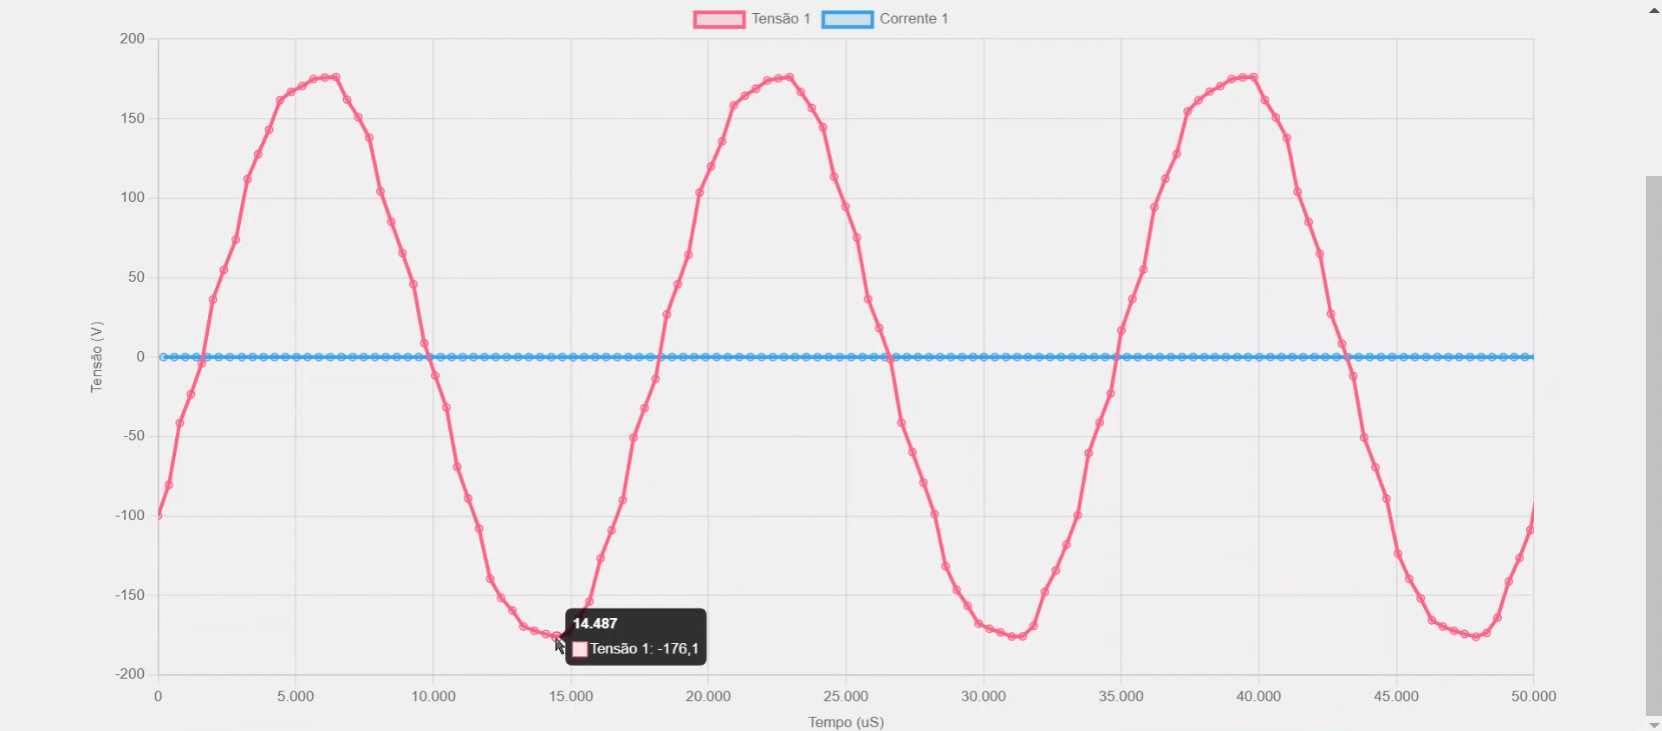
\includegraphics[width=\textwidth, height=\textheight, keepaspectratio]{webpage-tela2.png}
    \label{fig:webpage2}
    \fonte{}
\end{figure}

\subsubsection{Modularidade no Software}\label{modular-softw}

A comunicação foi testada utilizando-se dois módulos \textit{ESP32} e dados pré-programados de leitura, permitindo que fosse possível estabelecer o conceito da comunicação e elaborar a máquina de estados que define como a comunicação precisa ser tratada.

\begin{figure}[h!]
    \centering
    \caption{Máquina de Estados Completa}
    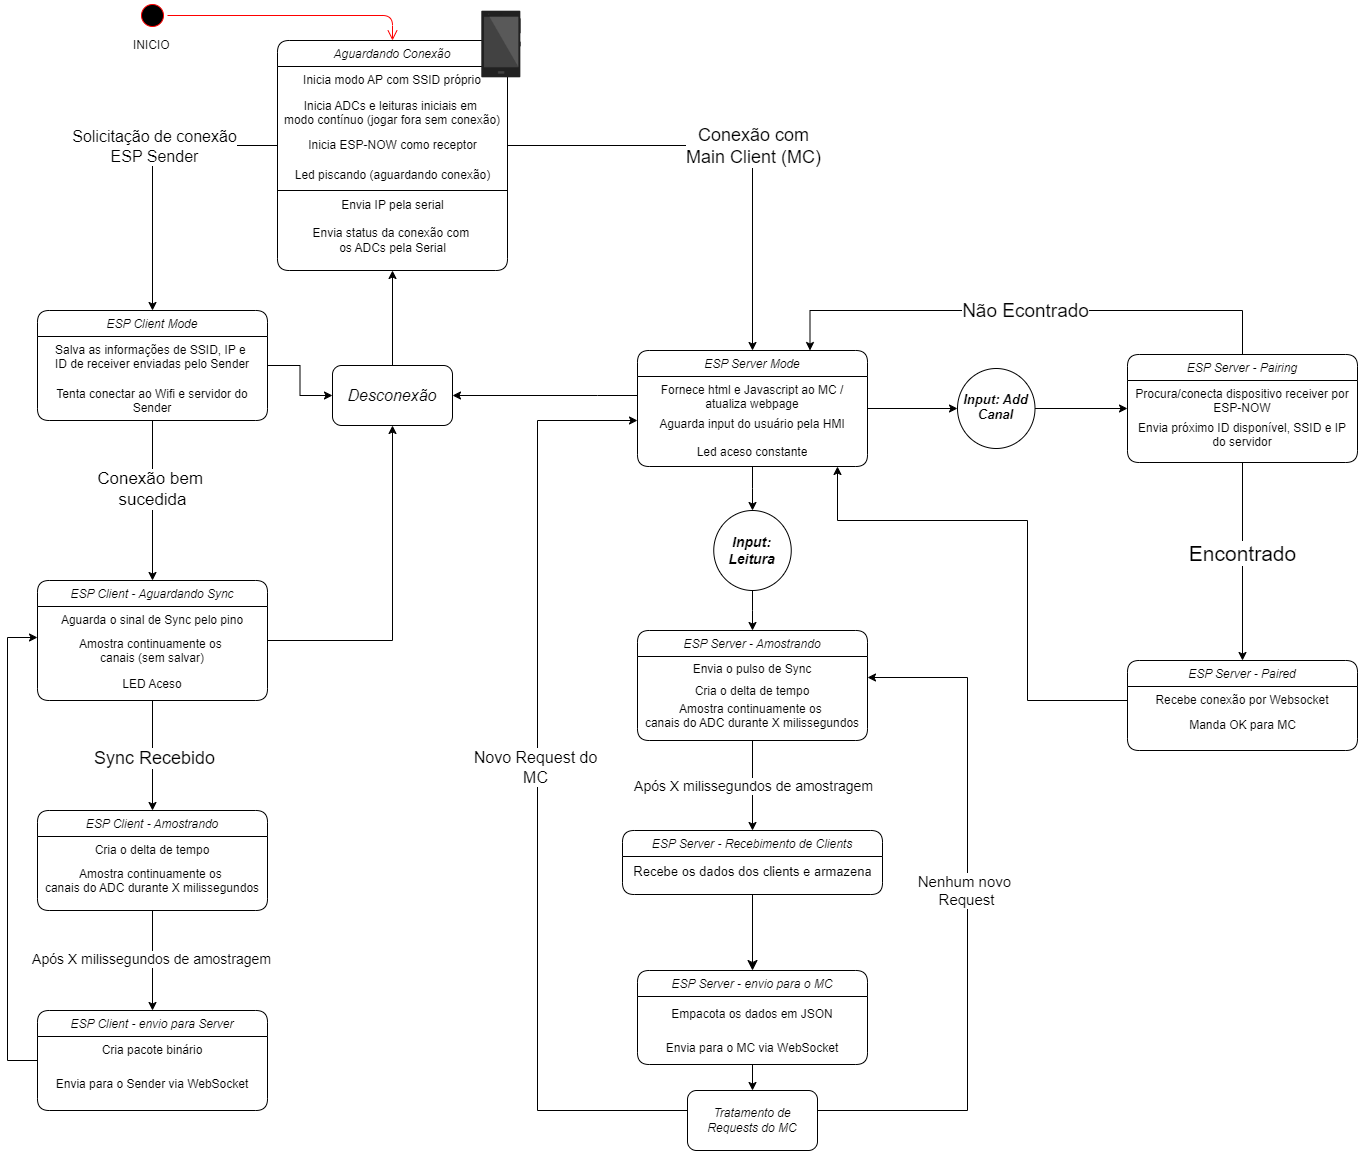
\includegraphics[width=\textwidth, height=\textheight, keepaspectratio]{state-machine-complete.png}
    \label{fig:maq-estados-completa}
    \fonte{}
\end{figure}

É possível observar pela \autoref{fig:maq-estados-completa} que sua implementação torna o código e o desenvolvimento desse trabalho extremamente complexos.

Após o processo da máquina de estados padrão, apresentada na \autoref{fig:maq-estado-simp} - com a modularidade futuramente implementada - o funcionamento da máquina de estados completa se daria da seguinte forma:
\begin{enumerate}
    \item Caso o cliente deseje adicionar um canal de leitura, o microcontrolador utiliza o protocolo \textit{ESP-NOW} para procurar e parear com um dispositivo adicional disponível.
    
    \item Assim, após o emparelhamento bem-sucedido, estabelece-se uma relação de \textit{client} com o dispositivo adicional, fornecendo-lhe todas as informações da rede necessárias para que ele acesse a mesma \textit{webpage} e \textit{Websocket}.
    
    \item Nesse momento, o uso do protocolo \textit{ESP-NOW} é finalizado, e toda a comunicação subsequente é realizada diretamente via \textit{Websocket}. Isso reduz a carga de processamento no microcontrolador e otimiza o tempo de comunicação e a transmissão de dados, pois o tamanho dos pacotes aumenta de 255 bytes para até 5 kilobytes
    
    \item Ao iniciar uma nova leitura via \textit{input} do cliente, um sinal de \textit{sync} é enviado do servidor \textit{master} para o módulo do canal adicional, estabelecendo assim uma referência temporal para sincronizar as leituras. A adição de canais é limitada a dois, permitindo a leitura trifásica.
\end{enumerate}

\subsection{Dificuldades encontradas e trabalhos futuros}\label{dificuldades-futuro}

Devido a dificuldades durante o desenvolvimento do projeto, não foi possível implementar por completo a função de modularidade entre os dispositivos. Dessa maneira, não é possível observar mais de um módulo ao mesmo tempo com o protótipo desenvolvido.

\subsubsection{ADC falsificado}\label{adc-falso}

Um grande empecilho encontrado foi a não conformidade do \gls{ADC} adquirido para a confecção do protótipo. Esse foi comprado de forma online em uma loja com baixa reputação e, como consequência, possuía sua velocidade de leitura fixada a menos que 500 \gls{SPS}. Devido a complexidade de desenvolvimento do firmware, muito foi testado até se chegar a conclusão de que o CI tratava-se de uma falsificação que não atendia o explicitado no datasheet do ADS1015. Esse foi posteriormente substituído por um de melhor procedência, alcançando os 3300 \gls{SPS} esperados sem maiores dificuldades.
Ao leitor, recomenda-se evitar o módulo indicado como cópia na \autoref{fig:adc-falsificado}, procurando sempre pelo original.

\begin{figure}[h!]
    \centering
    \caption{Comparação entre ADS1015 cópia e original}
    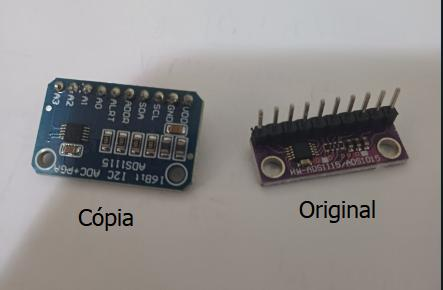
\includegraphics[width=\textwidth, height=\textheight, keepaspectratio]{figuras/adc-fake-comparison.jpeg}
    \label{fig:adc-falsificado}
    \fonte{}
\end{figure}

\subsubsection{Limitação do protocolo \textit{ESP-NOW}}\label{limit-espnow}

De início, foi considerada a utilização do protocolo \textit{ESP-NOW} para o envio de dados entre dispositivos. Visto que trata-se de um protocolo criado pela própria fabricante de microcontrolador utilizado, e possui vasta documentação de uso disponível.
Uma limitação desse protocolo, porém, é o tamanho máximo de 255 bytes por pacote de dados. Um par de pontos de tensão e corrente ocupa cerca de 160 bits, considerando a \textit{struct} apresentada na \autoref{tab:struct-graph}. Com essa limitação, é possível transmitir no máximo 12 pontos de uma forma de onda, o que é insuficiente, considerando que uma onda completa requer aproximadamente 55 pontos a uma taxa de 3300 \gls{SPS} e que, para uma análise adequada de uma rede trifásica, é necessário amostrar ao menos 3 ciclos de onda \cite{3ph-ozm}.
Como forma de contornar esse problema, seria necessária a implementação da comunicação entre módulos utilizando \textit{websockets}. O que tornou o desenvolvimento dessa etapa mais complexo do que o esperado.

\subsubsection{Isolamento entre canais}\label{isola-canais-dific}

Conforme discutido na \autoref{isolamento-metodologia}, o isolamento entre os canais de tensão e corrente foi necessário para o correto funcionamento do circuito. E pesquisas e testes para validação de propostas funcionais tomaram mais tempo do que o esperado.
Tal problema poderia ser contornado alterando alguns requisitos do projeto. 
Caso o dispositivo fosse projetado para ler apenas tensão e corrente alternadas, por exemplo, seria possível utilizar um transformador de corrente na respectiva entrada do \gls{ADC}, inerentemente isolando este canal do restante do circuito. 
Ou caso não fosse necessária a medição entre diferentes pontos do circuito - utilizando um ponto comum de medição, como mostrado na \autoref{fig:ponto-comum}. Seria possível manter ambos os canais na mesma referência, levando em consideração apenas o ruído transmitido de um canal para o outro.

\begin{figure}[h!]
    \centering
    \caption{Circuito de leitura simplificado utilizando ponto comum de referência}
    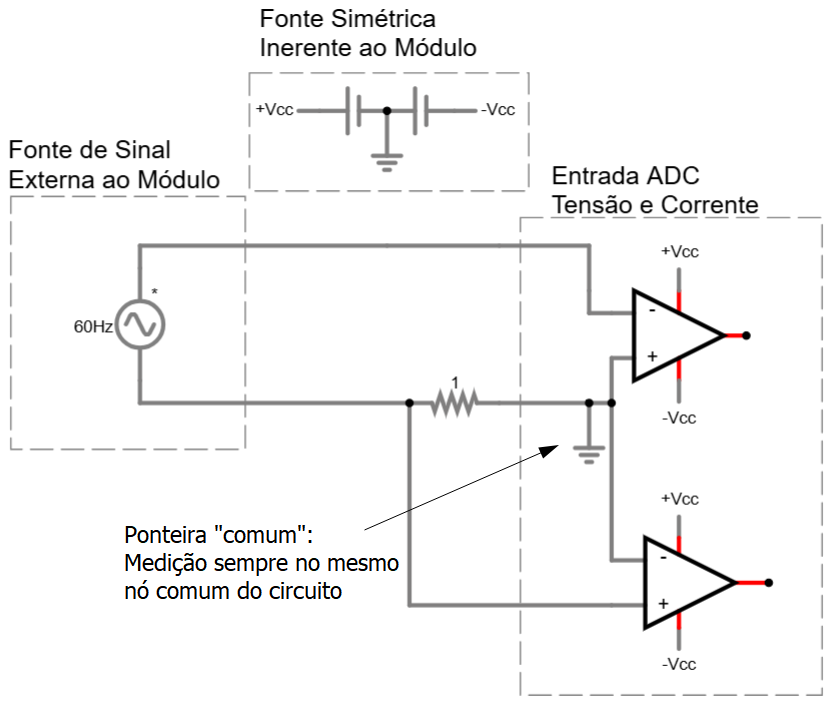
\includegraphics[width=\textwidth, height=\textheight, keepaspectratio]{figuras/diferencial-ponto-comum.png}
    \label{fig:ponto-comum}
    \fonte{}
\end{figure}

\section{Materiais}\label{sec:materiais}

Esta seção está dedicada à lista de materiais utilizados para a confecção de um protótipo. Os preços indicados são validos somente para a data de confecção desta monografia, pois estão cotados de acordo com o que se foi pago para a confecção deste, sendo os componentes originados de várias lojas diferentes, online e físicas, na China e no Brasil e também em datas diferentes.

Nota-se também que para efeito de testes e de montagem do protótipo testado, não se foi considerada a proteção de entrada por dois fatores: primeiramente esta é extremamente cara e difícil de encontrar (em questão aos fusíveis). Outro motivo é a segurança dos autores, pois testes de proteção são perigosos necessitam aparatos especiais.

\begin{table}[h!]
\centering
\caption{Lista de Materiais e Custos}
\label{tab:Bookofmaterials}
\begin{tabular}{|l|c|c|c|}
\hline
\textbf{Material} & \textbf{Quantidade} & \textbf{Preço por Unidade (R\$)} & \textbf{Valor Total (R\$)} \\ \hline
ESP32 & 1 & 60,00 & 60,00 \\ \hline
ADC ADS1015 & 2 & 35,00 & 70,00 \\ \hline
Buzzer THT & 1 & 3,50 & 3,50 \\ \hline
Capacitor 100 nF & 16 & 0,25 & 4,00 \\ \hline
Capacitor 330 pF & 4 & 0,15 & 0,60 \\ \hline
Capacitor 10 µF & 4 & 0,20 & 0,80 \\ \hline
Capacitor 1 µF & 6 & 0,20 & 1,20 \\ \hline
Diodo Schottky 1N5819 & 4 & 0,25 & 1,00 \\ \hline
Diodo 1N4007 & 10 & 0,15 & 1,50 \\ \hline
Trimpot 1 K$\Omega$ & 4 & 3,60 & 14,40 \\ \hline
Transistor BC547 & 1 & 0,25 & 0,25 \\ \hline
Resistor 220 $\Omega$ & 6 & 0,10 & 0,60 \\ \hline
Resistor 1 k$\Omega$ & 13 & 0,10 & 1,30 \\ \hline
Resistor 330 $\Omega$ & 2 & 0,10 & 0,20 \\ \hline
Resistor 0 $\Omega$ & 4 & N/A & 0,00 \\ \hline
Resistor 3k3 $\Omega$ & 1 & 0,10 & 0,10 \\ \hline
Resistor 1\% 2 M$\Omega$ & 4 & 0,08 & 0,32 \\ \hline
Resistor 1\% 10 k$\Omega$ & 4 & 0,10 & 0,40 \\ \hline
Resistor 1\% 100 $\Omega$ & 4 & 0,20 & 0,80 \\ \hline
Resistor 1\% 1 $\Omega$ & 4 & 0,20 & 0,80 \\ \hline
Resistor SMD 1\% 10 m$\Omega$ & 1 & 0,30 & 0,30 \\ \hline
Varistor S05K385 & 2 & 3,00 & 6,00 \\ \hline
Fusível HRC 440 mA & 1 & 45,50 & 45,50 \\ \hline
Fusível HRC 11 A & 1 & 49,50 & 49,50 \\ \hline
Borne KRE2 & 3 & 1,30 & 3,90 \\ \hline
Borne KRE3 & 2 & 2,00 & 4,00 \\ \hline
Chave Alavanca 2 posições & 1 & 4,20 & 4,20 \\ \hline
LM317T & 2 & 2,30 & 4,60 \\ \hline
LM358 & 2 & 1,10 & 2,20 \\ \hline
LM7805 & 2 & 1,60 & 3,20 \\ \hline
6N137 & 5 & 3,20 & 16,00 \\ \hline
Barra de Pinos Fêmea 40x1 & 2 & 3,10 & 6,20 \\ \hline
Fonte Isolada & 2 & 12,50 & 25,00 \\ \hline
\textbf{TOTAL} &  &  & \textbf{332,37} \\ \hline
\end{tabular}
\end{table}


\section{\textit{Casing}}\label{Casing}

Para a confecção do invólucro, ou \textit{casing} do protótipo, foi utilizado uma plataforma também gratuita de modelagem, chamada \textit{Onshape}.

Foram tiradas as medidas de um módulo de bancada de madeira, que suporta os equipamentos em bancadas dos laboratórios em questão, como demonstrado na \autoref{fig:Modulo-Base-Frente} e então feito o design com estas e também respeitando o tamanho e configuração da \gls{PCB}.

\begin{figure}[htb!]
    \caption{Módulo de Bancada}
    \label{fig:Modulo-Base-Frente}
    \includegraphics[width=0.8\textwidth]{figuras/Modulo-Base-Frente.jpg}
    \fonte{}
\end{figure}

O modelo foi pensado para ser o mais simples possível de ser impresso em 3D e modificado. Possui espaço para a placa e periféricos necessários.
Devido a dificuldades no desenvolvimento do trabalho, o encapsulamento não foi fabricado, apenas teve seu dimensional analisado em ambiente virtual.
Uma visão geral do modelo pode ser visto na \autoref{fig:osciloboy-isometrico}, juntamente de uma representação simplificada do suporte de madeira citado anteriormente.
O detalhe dos suportes internos pode ser visto na \autoref{fig:osciloboy-detalhes}.

\begin{figure}[htb!]
    \caption{Modelo virtual do encapsulamento}
    \label{fig:osciloboy-isometrico}
    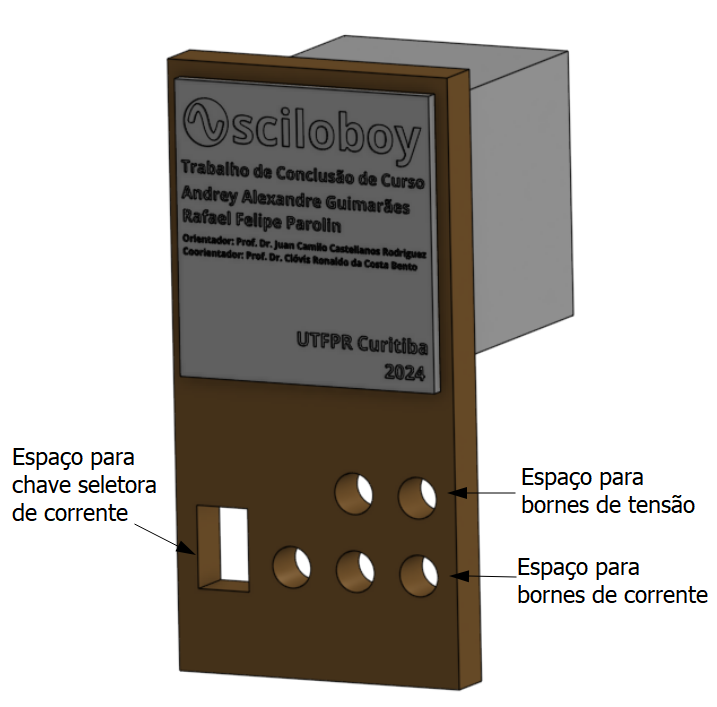
\includegraphics[width=0.8\textwidth]{figuras/osciloboy-case-1.png}
    \fonte{}
\end{figure}

\begin{figure}[htb!]
    \caption{Detalhes de suportes para PCB e periféricos}
    \label{fig:osciloboy-detalhes}
    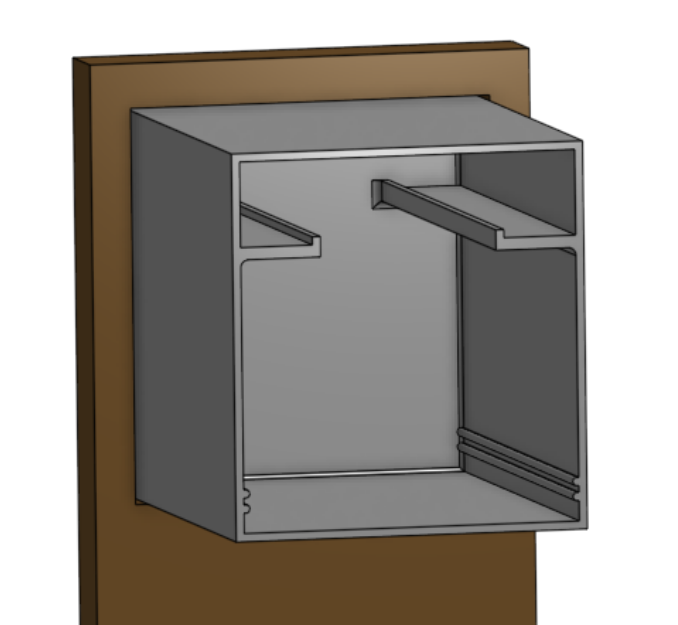
\includegraphics[width=0.8\textwidth]{figuras/osciloboy-case-2.png}
    \fonte{}
\end{figure}

Assim como os demais elementos desse projeto, pode ser encontrado no [APENDICE X -TODO-] ao final do trabalho, bem como, dado a característica colaborativa da plataforma, pode ser clonado e modificado sem nenhum custo, conforme a necessidade do usuário.